\documentclass[10pt]{jarticle}
%T \usepackage{newtxtext,newtxmath}
\usepackage{url}
\usepackage{pcsjimps-j}
\usepackage[dvipdfmx]{graphicx}
\usepackage[dvipdfmx,bookmarks=false]{hyperref}

\begin{document}
\pagestyle{empty}

\twocolumn[\centering
% 日本語タイトル
\JTitle{画像符号化シンポジウム・映像メディア処理シンポジウム\\講演予稿の書き方}
% 英語タイトル
\ETitle{How to Prepare a Camera-Ready Paper for Picture Coding Symposium of Japan and
Image Media Processing Symposium}

% 著者
\JEAuthor{和文著者1$^\dag$}{Author 1$^\dag$}{30mm}
\JEAuthor{和文著者2$^\ddag$}{Author 2$^\ddag$}{30mm}
\JEAuthor{和文著者3$^\dag$}{Author 3$^\dag$}{30mm}\\
% 所属
\JEAffiliation{$^\dag$PCSJ/IMPS実行委員会}{$^\dag$PCSJ/IMPS Organizing Committee}{70mm}
\JEAffiliation{$^\ddag$和文所属2}{$^\ddag$English Affiliation 2}{50mm}\\

% 概要
\Abstract{
内容を300字程度で記述します。内容を300字程度で記述します。
内容を300字程度で記述します。内容を300字程度で記述します。
内容を300字程度で記述します。内容を300字程度で記述します。
内容を300字程度で記述します。内容を300字程度で記述します。
内容を300字程度で記述します。内容を300字程度で記述します。
内容を300字程度で記述します。内容を300字程度で記述します。
内容を300字程度で記述します。内容を300字程度で記述します。
内容を300字程度で記述します。内容を300字程度で記述します。
内容を300字程度で記述します。内容を300字程度で記述します。
内容を300字程度で記述します。
}
]

%本文

\section{はじめに}

%S 本PDFはドキュメントクラスjsarticleのサンプルです。

%T 本PDFはドキュメントスタイルnewtxのサンプルです。


講演予稿集は、USBおよび印刷物(白黒)により出版致します。
提出は、PDFファイルを指定サイトへアップロードいただきます。

特別講演は
フォーマット自由、ページ制限無し(8ページ程度以内)。
予稿集では顔写真と略歴を先頭ページに記載します。

本サンプルは\underline{一般講演}の説明になります。

\vspace{5cm}

\section{分量、原稿サイズ}

\begin{itemize}
\item 1件2ページ以内(図表を含む)
\item A4サイズ
\item 幅180mm
\item 高さ252mm
\item 段間の幅8mm程度(二段組の場合)
\end{itemize}
としてください。

\vspace{5cm}

\section{配置}


\begin{itemize}
\item 表題、著者名、勤務先は、本サンプルに従ってそれぞれ記入して下さい。
\item アブストラクト(和文の場合300字程度、英文の場合100語程度)をお入れ下さい。
\item 本文は一段または左右二段に書いても差し支えありません。
\item 用紙最終頁右下に、発表者連絡先をお入れ下さい(本サン
      プルのマクロ\verb|\simplefootnotetext|を使われると便利です)。
\end{itemize}



\section{文字サイズ}
文字サイズは、本サンプルを目安にしてください。
\begin{description}
\item[表題] 16ポイント (\verb|\LARGE|)
\item[和文著者名] 14ポイント(\verb|\Large|)
\item[英文著者名] 12ポイント(\verb|\large|)
\item[所属および本文] 10ポイント(\verb|\normalsize|)
\end{description}
程度です。

\section{図表}

\begin{table}[tb]
\caption{符号化器の設定}
\label{tab:settings}
\centering
\begin{tabular}{c||c|c}\hline
設定ア & aa & aaa\\\hline
設定イ & bb & bbb\\\hline
設定ウ & cc & ccc\\\hline
\end{tabular}
\end{table}

\begin{figure}[tb]
\centering
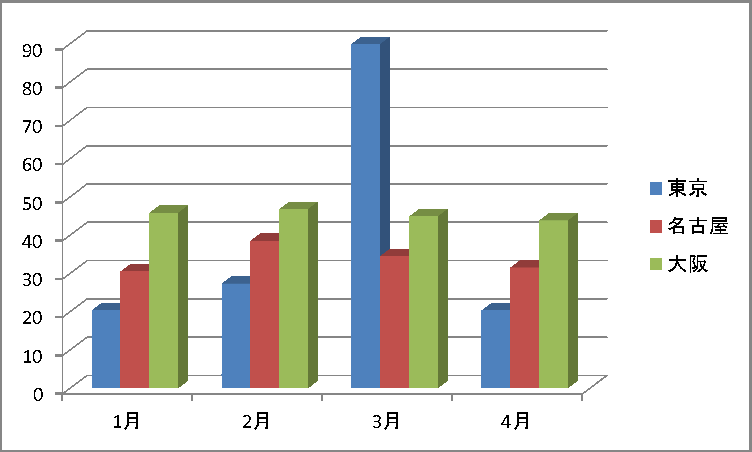
\includegraphics[width=.55\columnwidth]{./sample-j.eps}\\
\caption{符号化実験結果}
\label{fig:results}
\end{figure}


予稿集は白黒・網がけ印刷になります。見にくくならないよう、作成の際には
ご注意ください。

図表の出力位置を指定するオプションは、[h]は使わず[t]、[b]などを指定して
ページの天か地に置くことを基本にします。

図表内は英文でも和文でも結構です。
参照は図\ref{fig:results}、表\ref{tab:settings}のようにしてください。

\vspace{5cm}

\section{PDFファイル化}
PDF作成時はすべてのフォントを埋め込むように設定して下さい。
AcrobatやWeb上のフリーのツール等で構いませんので、必ずフォント埋め込みを確認して下さい。

変換コマンド例は以下の通りです:
\begin{verbatim}
$ platex foo.tex
$ dvipdfmx -p a4 foo.dvi
または
$ simpdftex platex --mode dvipdfmx --dvipdfmopts \
  "-p a4" foo.tex
\end{verbatim}


\section{その他\LaTeXe 特有の事項}

お好みでnewtx\cite{newtx}やjsclasses\cite{jsclasses}を用い、より美し
い組版をしていただいても構いません。

%T \def\egstr{{\it Font Example}, Bj\o ntegaard delta, {\it Karsten S\"uhring}}
%T txfontによるTimes-Romanフォントと
%T 通常の\TeX フォント(Computer Modern Roman)を順に示します:\\
%T \egstr\\
%T {\renewcommand{\rmdefault}{cmr}\normalfont \egstr}


原則として半角に存在する文字については全角を使わないようにします(e.g., 
``(ABC123)''は``(ABC123)''のように)。

半角と全角の間にスペースを入れる(e.g., \verb*|10 種類|)必要はあ
りません(自動的に四分アキが入ります(10種類))。

p\LaTeXe コンパイル時のフォントに関するWarningを抑制するにはjtygmスタイ
ルファイル\cite{jtygm}をご参考にされてください。

参考文献等でのURLの表記には、urlスタイルファイルを使い
\verb|\url{http://...}|とされると便利です。
また、同URLにハイパーリンクを付与するにはhyperref を利用します
\cite{mizutani}。

その他、
\LaTeX のコマンド・パッケージの使用方法について、
\cite{maruta}の情報が参考になります。

\section{おわりに}
平成19年3月2日 初版\par
平成19年3月8日 更新\par
平成26年5月23日 更新\par
平成27年7月15日 更新

\def\etal{{\it et al.}}
\begin{thebibliography}{9}
 \bibitem{CALIC} X. Wu \etal: ``Context-based, adaptive, 
	 lossless image codec,'' IEEE Trans. Commun., vol. 45, pp. 437--444, 
	 Apr. 1997
 \bibitem{newtx}
	 M. Sharpe: ``newtx -- Alternative uses of the TX fonts, with improved metrics'',
         \url{http://www.ctan.org/pkg/newtx}
 \bibitem{jsclasses}
         奥村晴彦: ``p\LaTeXe 新ドキュメントクラス'',
         \url{http://oku.edu.mie-u.ac.jp/~okumura/jsclasses/}
 \bibitem{jtygm}
         堀田耕作: ``jtygmスタイルファイル'',
         \url{http://www.khotta.org/ghost/psfont.html}
 \bibitem{mizutani}
         水谷正大: ``ハイパーリンク付きLaTeX文書'',	 
	 \url{http://www.isc.meiji.ac.jp/~mizutani/tex/link_slide/hyperlink.html}
 \bibitem{maruta}
         丸田一郎: ``使ってはいけない\LaTeX のコマンド・パッケージ・作法'',
         \url{http://ichiro-maruta.blogspot.jp/2013/03/latex.html}
\end{thebibliography}

\simplefootnotetext{
○○研究所 ××プロジェクト\\
〒\hspace{0pt}222--2222 ○○市××町1-1-1\\
Phone: 000-111-2222, Fax: 000-111-2223\\
E-mail:  foo@example.jp}
\end{document}
